\subsection{Front-end}

\hspace{0.5cm} Użytkownicy będą korzystali z naszej aplikacji za pośrednictwem strony internetowej. Nawigacja po niej będzie realizowana poprzez zastosowanie paska nawigacyjnego na górze ekranu. Dzięki niemu będzie można przejść między innymi do rejestracji i logowania. Po rejestracji i zalogowaniu do systemu użytkownik będzie mógł przejść do następujących komponentów:
\begin{itemize}

    \item strona główna - będzie zawierała najważniejsze informacje dotyczące wykupionych przez niego subskrybcji
    \item profil użytkownika - komponent, w którym będą zebrane informacje o koncie zalogowanego użytkownika
    \item zakup subskrypcji - miejsce, w którym użytkownik będzie mógł nabyć nową subskrypcję
    \item statystki - komponent, gdzie będzie zbiorcze zestawienie danych dotyczących wszystkich subskrypcji użytkownika
\end{itemize}
\begin{center}
    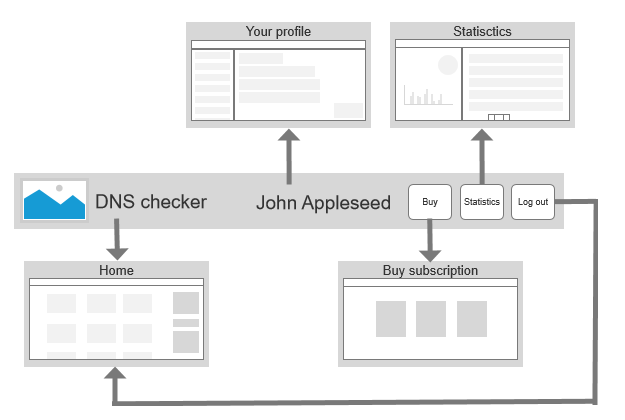
\includegraphics[scale=0.75]{sitemap.png}
\end{center}
